\documentclass[compress]{beamer}
\usepackage{multirow}
\newcommand{\argmin}{\operatornamewithlimits{argmin}}
\def\qeq{\mathrel{%
    \mathchoice{\QEQ}{\QEQ}{\scriptsize\QEQ}{\tiny\QEQ}%
}}
\def\QEQ{{%
    \setbox0\hbox{$\sim$}%
        \rlap{\hbox to \wd0{\hss!\hss}}\box0
}}

\usetheme{Warsaw}
\setbeamertemplate{navigation symbols}{}
\useoutertheme[footline=authortitle,subsection=false]{miniframes}
\title[Exploring Topic Coherence over many models and many topics]
      {Exploring Topic Coherence over many models and many topics}

\author[Stevens, Kegelmeyer, Andrzejewski, Buttler]
       {Keith Stevens \inst{1} \inst{2} \and 
        Philip Kegelmeyer \inst{3} \and \\
        David Andrzejewski \inst{1} \and
        David Buttler \inst{1}}
\institute{\inst{1} Lawrence Livermore National Lab \and
           \inst{2} University of California, Los Angeles \and 
           \inst{3} Sandia National Lab
\thanks{
    \tiny
This work was performed under the auspices of the U.S. Department of Energy by
Lawrence Livermore National Laboratory under Contract DE-AC52-07NA27344
(LLNL-XXXX-XXXXXX) and by Sandia National Laboratory under Contract
DE-AC04-94AL85000.}
           }

\date{}

\begin{document}

\frame{
    \titlepage
}

\section{Motivation}

\begin{frame}{Why Learn Topic Models?}

\begin{columns}
\begin{column}[1]{5cm}
Suppose you're given a lot of articles to read:

\includegraphics[width=.50\textwidth,height=.30\textwidth]{figures/the_new_york_times_logo_8983D9A61EC52.jpg}

\includegraphics[width=.40\textwidth,height=.30\textwidth]{figures/Wikipedia-logo.png}
\end{column}
\begin{column}[2]{5cm}
Questions:
\begin{itemize}
\item How do you grok the corpus?
\item How do you discover relevant events?
\item How do you make these tasks easy?
\end{itemize}
\end{column}
\end{columns}

\pause
\begin{block}{Bjarne Stroustrup}
A high level of abstraction is good
\end{block}

\pause
\begin{itemize}
\item Abstraction reduces the complexity of a dataset
\item Topic models learn good abstractions 
\end{itemize}
\end{frame}

\begin{frame}{Testing the value of learned abstractions}
\begin{block}{Intuition: Topics correspond to concepts, sort of}
\begin{enumerate}
\item Topics represent distinctions matching human intuition
\item Uncovered Topics reduce complexity when comparing words and documents
\end{enumerate}
\end{block}

\begin{overlayarea}{\textwidth}{4cm}
\only<2>{
    All three models are used interchangeably:
    \begin{itemize}
    \item Word Similarity Judgements (Reisinger \& Mooney 11, Jurgens+ 10)
    \item Document Classification (Mimno+ 09, Foltz \& Dumais 92)
    \item Information Retrieval (Andrzejewski \& Buttler 11, Hoffman 99, etc)
    \end{itemize}
    $ \rightarrow $ Time to compare all three again \\
}
\only<3>{
\pause
Big Question: Why/When Should We Use Particular Models?
\begin{enumerate}
\item How do you evaluate an entire model?
\item Is one model strictly better than other?
\item Does each model specialize for a task?
\end{enumerate}
}
\only<4->{
\pause
Three Evaluations testing our intuitions and questions:
\begin{enumerate}
\item Compactly evaluate quality of both topics and entire models
\item Compare abstracted word representations to topic coherence
\item Compare abstracted document representations to topic coherence
\end{enumerate}
\pause
Core Question: does semantic quality of a topic model indicate that the model
has good abstract representations?
}
\end{overlayarea}
\end{frame}

\begin{frame}{Outline}
\begin{enumerate}
\item Motivation for modeling semantics
\item Topic Models
    \begin{enumerate}
    \item A shared framework
    \item Latent Dirichlet Allocation
    \item Decompositional approaches
    \end{enumerate}
\item Topic Coherence Metrics
    \begin{enumerate}
    \item Purpose
    \item Two measures of coherence
    \end{enumerate}
\item Comparing three evaluations
   \begin{enumerate}
   \item Evaluating complete models
   \item Evaluating semantic judgements
   \item Evaluating document categories
   \end{enumerate}
\item Conclusions
\end{enumerate}
\end{frame}

\section{Topic Models}

\subsection{A shared framework}

\begin{frame}{The Big Topic Modeling Picture}
\center
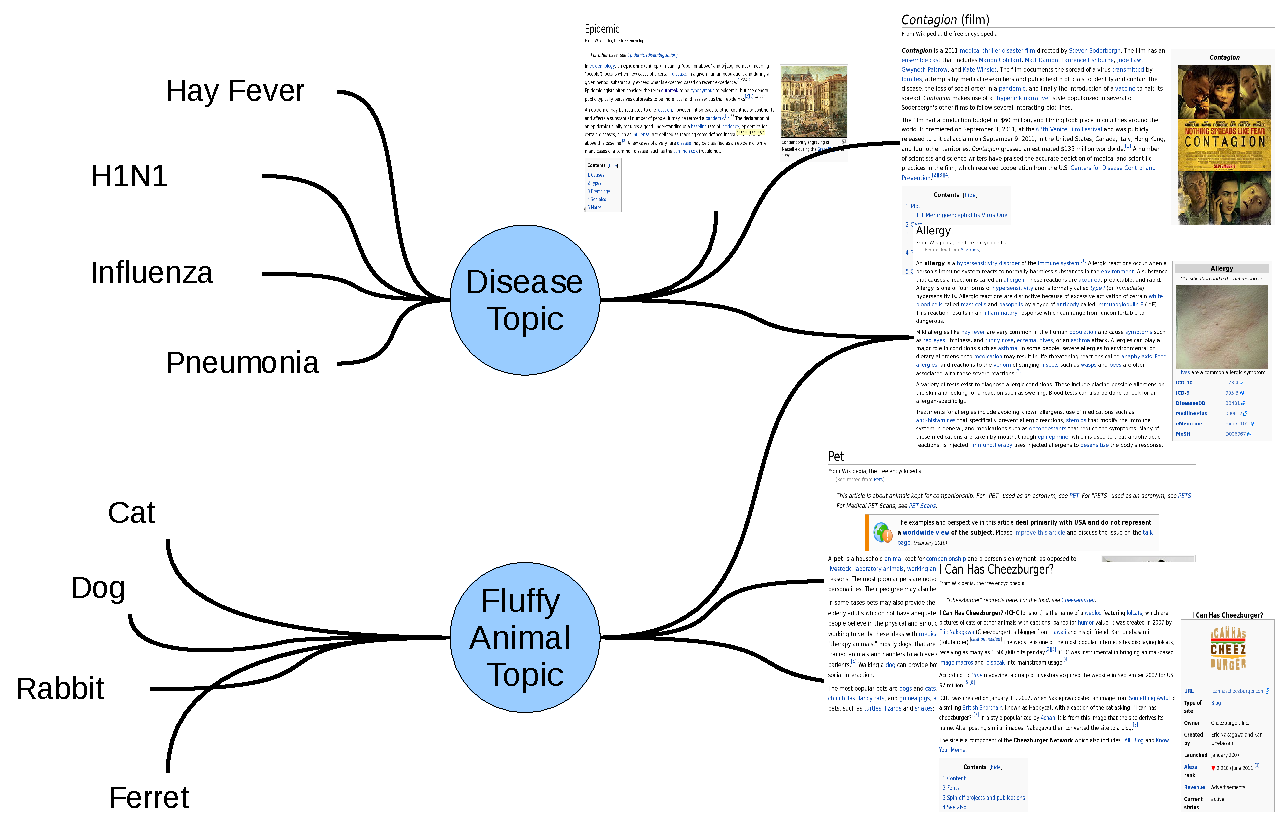
\includegraphics[width=.80\textwidth,height=.40\textwidth]{figures/topic-connection.pdf}

Topic Models learn latent factors that
\begin{enumerate}
\item Link together related Words
\item Link together related Documents
\item Link words to documents
\item Represent a semantic "concept"
\end{enumerate}
\end{frame}

\begin{frame}{A basic framework for Topic Models}
\begin{block}{Input}
A large collection of English documents such as New York Times articles
\end{block}

\begin{block}{Output}
Two Matrices:
\begin{itemize}
\item W records the strength between words and topics
\item H records the strength between documents and topics
\end{itemize}
Together, W and H should abstractly summarize the semantic content of the input
\end{block}
\end{frame}

\subsection{Latent Dirichlet Allocation}

\begin{frame}{A generative story for topics}
\begin{block}{Latent Dirichlet Allocation}
To "write" a document
\begin{enumerate}
\item Choose a mixture of topics for the document
\item For each word to write
    \begin{enumerate}
    \item Pick a topic from your mixture
    \item Write down a word from the topic
    \end{enumerate}
\end{enumerate}
\end{block}

\begin{columns}
\begin{column}[1]{6cm}
\begin{itemize}
\item $\theta$ represents how each document generates topics ($H$)
\item $\varphi$ represents how each topic generates words ($W'$)
\end{itemize}
\end{column}
\begin{column}[2]{4cm}
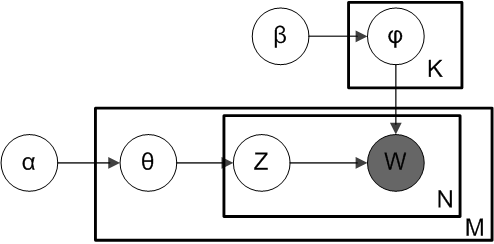
\includegraphics[width=.80\textwidth,height=.40\textwidth]{figures/Smoothed_LDA.png}
\end{column}
\end{columns}
\end{frame}

\subsection{A decompositional approach}

\begin{frame}{A story of decomposition for topics}
\begin{block}{Latent Semantic Analysis}
\begin{enumerate}
\item Form a Term X Document matrix (A)
\item Weight the counts to enhance informative words
\item Split the matrix along multiple, \textit{interesting} dimensions
\end{enumerate}
\end{block}

\begin{overlayarea}{\textwidth}{4cm}
\only<1>{
\begin{columns}
\begin{column}[1]{4cm}
The decomposition results in two matrices
\begin{itemize}
\item W: A Word by Topic matrix
\item H: A Document by Topic matrix
\end{itemize}
\end{column}
\begin{column}[2]{6cm}
The Source of generalization:
\begin{itemize}
\item Latent, interesting dimensions smooth the data
\item Smoothing flattens out noisy features
\end{itemize}
\end{column}
\end{columns}
}
\only<2>{
\pause
\begin{columns}
\begin{column}[1]{5.5cm}
Singular Value Decomposition:
\begin{itemize}
\item Decompose: $ A = U \Sigma V' $
\item Select top $k$ dimensions
\item Minimize Frobenius norm:
$ || A - U_k \Sigma_k V_k' ||^2 $
\item $ W = U_k \Sigma_k $, $ H = (\Sigma_k V_k')' $
\end{itemize}
\end{column}
\begin{column}[2]{5cm}
Features/Issues:
\begin{itemize}
\item Arbitrary latent dimensions
\item Possibly negative relationships
\item No Succinct interpretation
\end{itemize}
\end{column}
\end{columns}
}
\only<3>{
\pause
\begin{columns}
\begin{column}[1]{5.5cm}
Nonnegative Matrix Factorization:
\begin{itemize}
\item Decompose: $ A = W H' $
\item Minimize Frobenius norm:
$ || A - W H' ||^2 $
\item Enforce non-negative values
\end{itemize}
\end{column}
\begin{column}[2]{5cm}
Features/Issues:
\begin{itemize}
\item Decomposition forms probabilities
\item Easy to interpret
\item Approximated Solution
\end{itemize}
\end{column}
\end{columns}
}
\end{overlayarea}
\end{frame}

\section{Topic Coherence Metrics}

\subsection{Purpose}

\begin{frame}{The idea behind coherence metrics}
\begin{block}{Reminder: Topics correspond to concepts}
\begin{enumerate}
\item Topics represent distinctions matching human intuition
\item Uncovered Topics reduce complexity when comparing words and documents
\end{enumerate}
\end{block}
\begin{overlayarea}{\textwidth}{4cm}
\only<1>{
    Realization: \\
    $ correlation(perlexity, human\_intuition) \sim 0 $
}
\only<2>{
Evaluation Intuition: Words forming topics should be \textit{related}.
\[
Coherence(topic) = \sum_{w_1,w_2 \in topic} sim(w_1, w_2)
\]

$sim(w_i, w_j)$ returns the strength of \textit{relatedness} between two words.
}
\end{overlayarea}
\end{frame}

\subsection{Two measures of coherence}

\begin{frame}{Computing relatedness: An Intrinsic approach}
\begin{block}{UMass Topic Coherence}
\[
sim(w_i, w_j) = log \frac{ D(w_i, w_j) + \epsilon } { D(w_j) }
\]
\end{block}
High Level Idea:
\begin{itemize}
\item Measure frequency of words occurring the \textbf{same} document
\item Hi co-occurrence in relation to unigram occurrence = related
\end{itemize}

Key Detail: Compute counts on the training corpus.
\end{frame}

\begin{frame}{Computing relatedness: An Extrinsic approach}
\begin{block}{UCI Topic Coherence}
\[
sim(w_i, w_j) = log \frac{ p(w_i, w_j) + \epsilon } { p(w_i) p(w_j) }
\]
\end{block}

High Level Idea:
\begin{itemize}
\item Compute Pointwise Mutual Information between words
\item High PMI = related
\end{itemize}

Key Detail: Compute counts on representative, external corpus. \\
We used a 20 word sliding window on Wikipedia for our counts.
\end{frame}

\section{Comparing three evaluations}

\begin{frame}{Some sample learned topics}
\begin{table}[h!t!b!]
\center
\tiny
\begin{tabular}{|cll|}
\multicolumn{1}{c}{Model} & Label & \multicolumn{1}{l}{Top Words} \\
\hline
\multicolumn{3}{l}{\textbf{High Quality Topics}} \\
\hline
\multirow{2}{*}{LDA} 
% 500-32
& interview & told asked wanted interview people made thought time called knew
\\
% 500-176
& wine & wine wines bottle grapes made winery cabernet grape pinot red 
\\
\hline
\multirow{2}{*}{NMF} 
% 500-144
& grilling & grilled sweet spicy fried pork dish shrimp menu dishes sauce 
\\
% 500-120
& cloning & embryonic cloned embryo human research stem embryos cell cloning cells
\\
\hline
\multirow{2}{*}{SVD} 
% 500-5
& cooking & sauce food restaurant water oil salt chicken pepper wine cup 
\\
% 500-25
& stocks & fund funds investors weapons stocks mutual stock movie film show 
\\
\hline

\multicolumn{3}{l}{\textbf{Low Quality Topics}} \\
\hline
\multirow{2}{*}{LDA} 
% 500-290
& rates & 10-yr rate 3-month percent 6-month bds bd 30-yr funds robot 
\\
% 500-340
& charity & fund contributions .com family apartment charities rent 22d children assistance
\\
\hline
\multirow{2}{*}{NMF} 
% 500-76
& plants & stem fruitful stems trunk fruiting currants branches fence currant espalier 
\\
% 500-33
& farming & buzzards groundhog prune hoof pruned pruning vines wheelbarrow tree clematis
\\
\hline
\multirow{2}{*}{SVD} 
% 500-7
& city & building city area buildings p.m. floors house listed eat-in a.m.
\\
% 500-160
& time & p.m. system study a.m. office political found school night yesterday 
\\
\hline
\end{tabular}
\caption{Top 10 words from several high and low quality topics learned
automatically from 92,000 New York Times articles.}
\end{table}
\end{frame}

\begin{frame}{Experimental Setup}
\begin{block}{New York Times 2003 dataset}
\begin{itemize}
\item $\sim$ 92,000 articles, each with multiple section labels
\item Discard stop words, infrequent words ($< 200$ occurrences)
\item No Stemming
\end{itemize}
\end{block}

Three Topic Models: LDA, LSA using SVD, LSA using NMF \\
Many numbers of topics: 1-100, 100-500 in steps of 10.

\end{frame}

\subsection{Evaluating Complete Models}

\begin{frame}{Topic Coherence Measures}
\only<1>{
\begin{block}{Multiple ways of evaluating a complete model}
\begin{itemize}
\item Average Coherence
\item Best Coherence
\item Entropy of Coherence scores
\end{itemize}
\end{block}
}
\only<5>{
    \center
    Average UMass Topic Coherence with $\epsilon=10^{-12}$
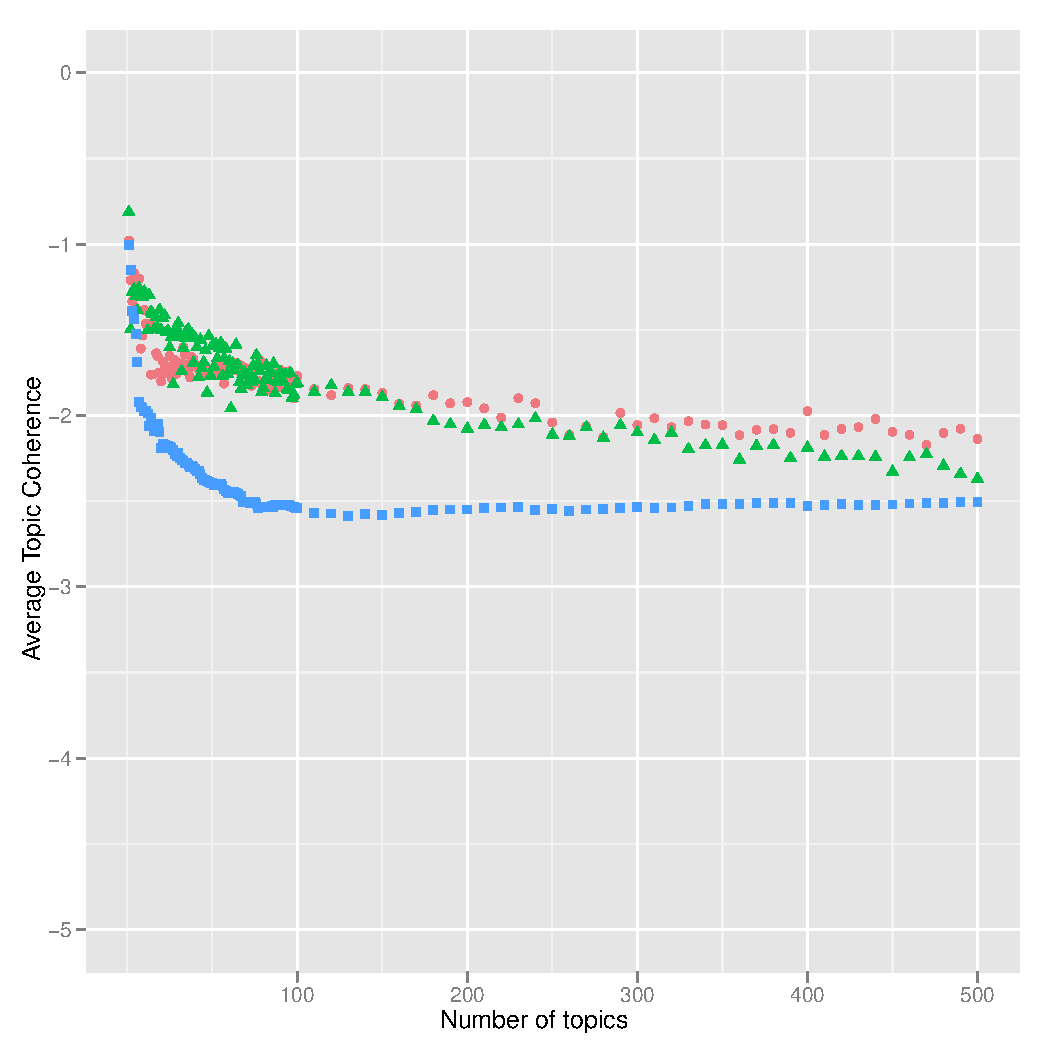
\includegraphics[width=\textwidth,height=.55\textwidth]{plots/mean-umassNoSmoothing.pdf}
}
\only<4>{
    \center
    Average UMass Topic Coherence with $\epsilon=10^{0}$
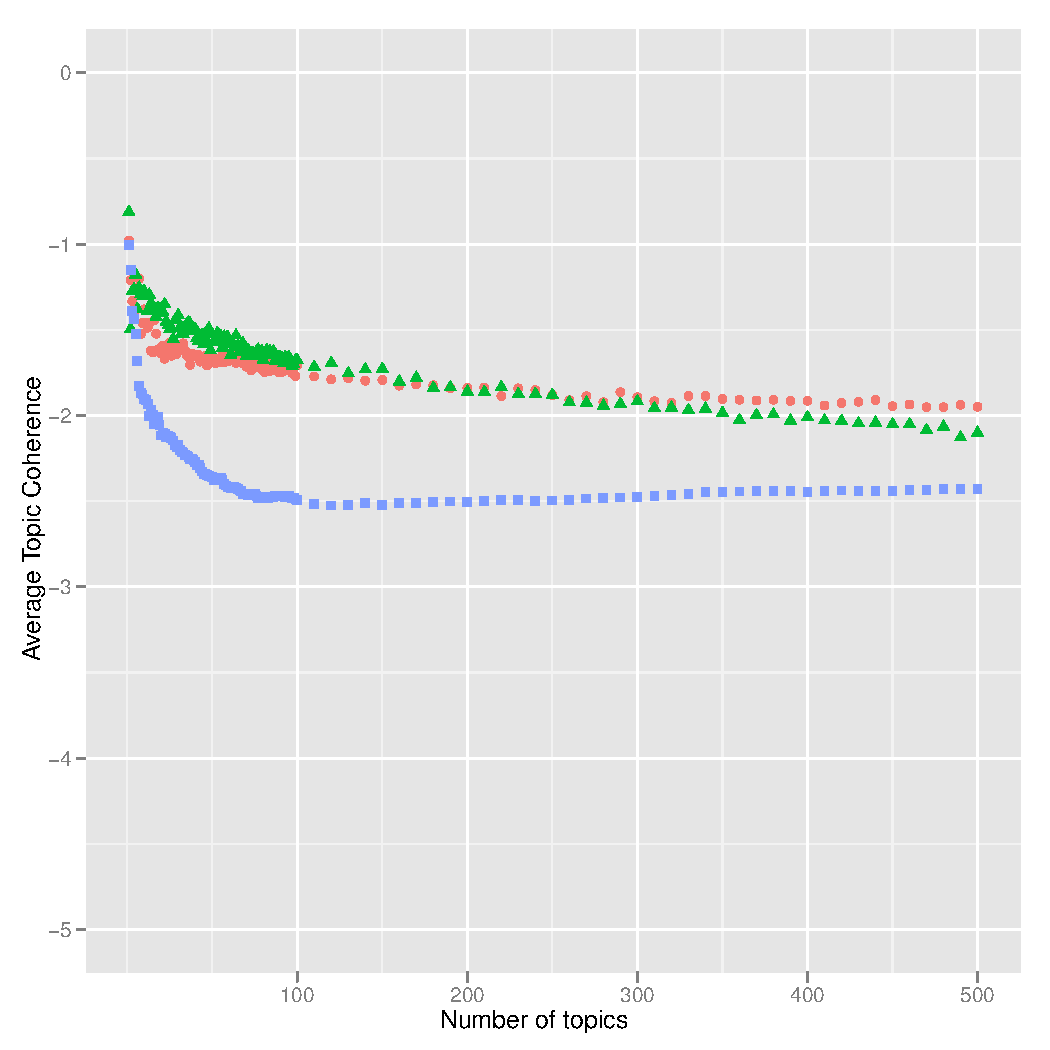
\includegraphics[width=\textwidth,height=.55\textwidth]{plots/mean-umass.pdf}
}
\only<3>{
    \center
    Average UCI Topic Coherence with $\epsilon=10^{-12}$
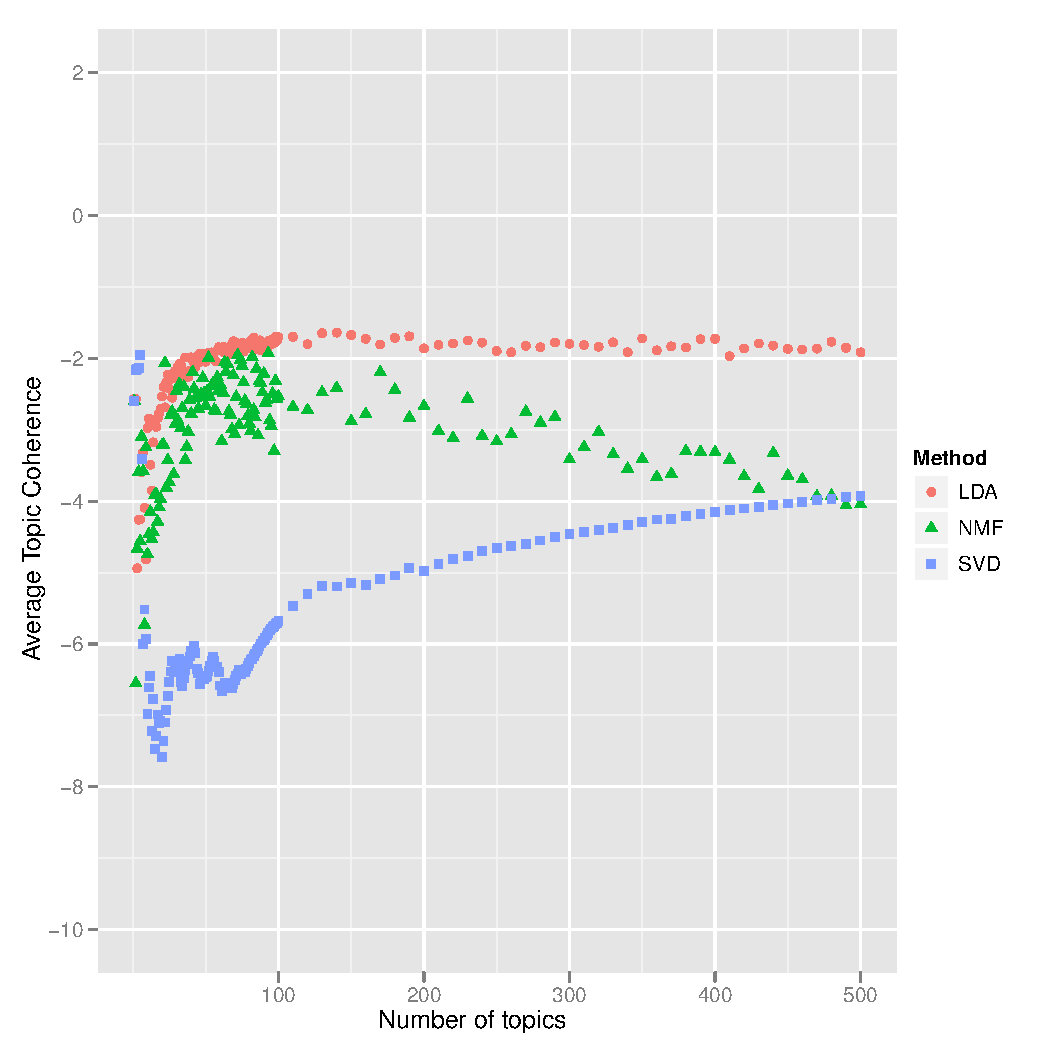
\includegraphics[width=\textwidth,height=.55\textwidth]{plots/mean-uciNoSmoothing.pdf}
}
\only<2>{
    \center
    Average UCI Topic Coherence with $\epsilon=10^{0}$
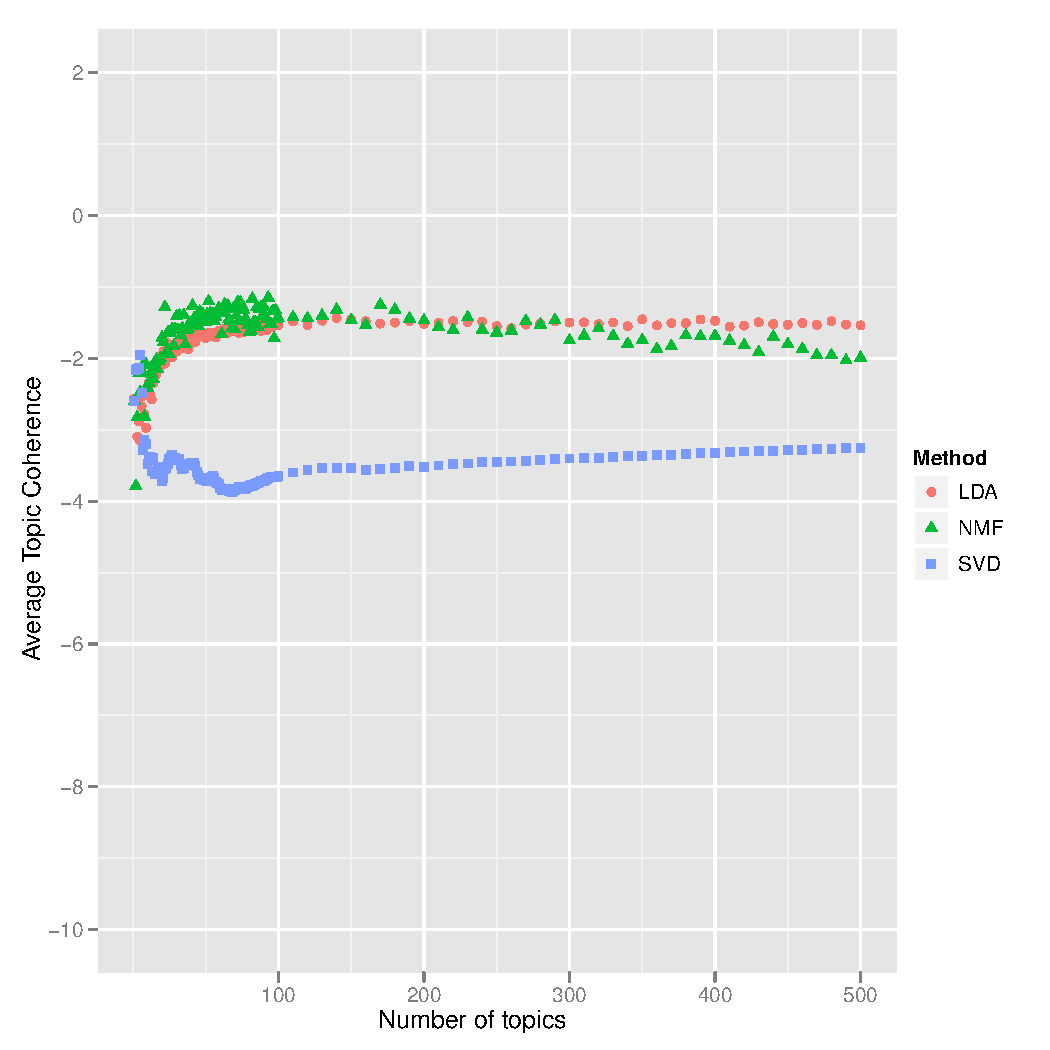
\includegraphics[width=\textwidth,height=.55\textwidth]{plots/mean-uci.pdf}
}
\end{frame}

\subsection{Evaluating semantic judgements}

\begin{frame}{Evaluating the latent word representations}

\only<1>{
\begin{block}{Humans are good at judging relatedness}
Example: $cat \sim dog$, $cat \qeq umbrella$ \\
Goal: Word representations should approximate human judgements
\end{block}

\begin{columns}
\begin{column}[1]{5cm}
\begin{tabular}{lll}
Word  & Word & Relatedness \\
\hline
coast & forest & 0.85 \\
monk & oracle & 0.91 \\
fruit & furnace & 0.05 \\
cord & smile & 0.02 \\
\hline
\end{tabular}
\end{column}
\begin{column}[2]{5cm}
\begin{enumerate}
\item Compute cosine similarity between latent word representations
\item Compute correlation between similarity measures and human judgements
\end{enumerate}
\end{column}
\end{columns}
}
\only<2>{
\center
Correlation with Rubenstein \& Goodenough word pairs
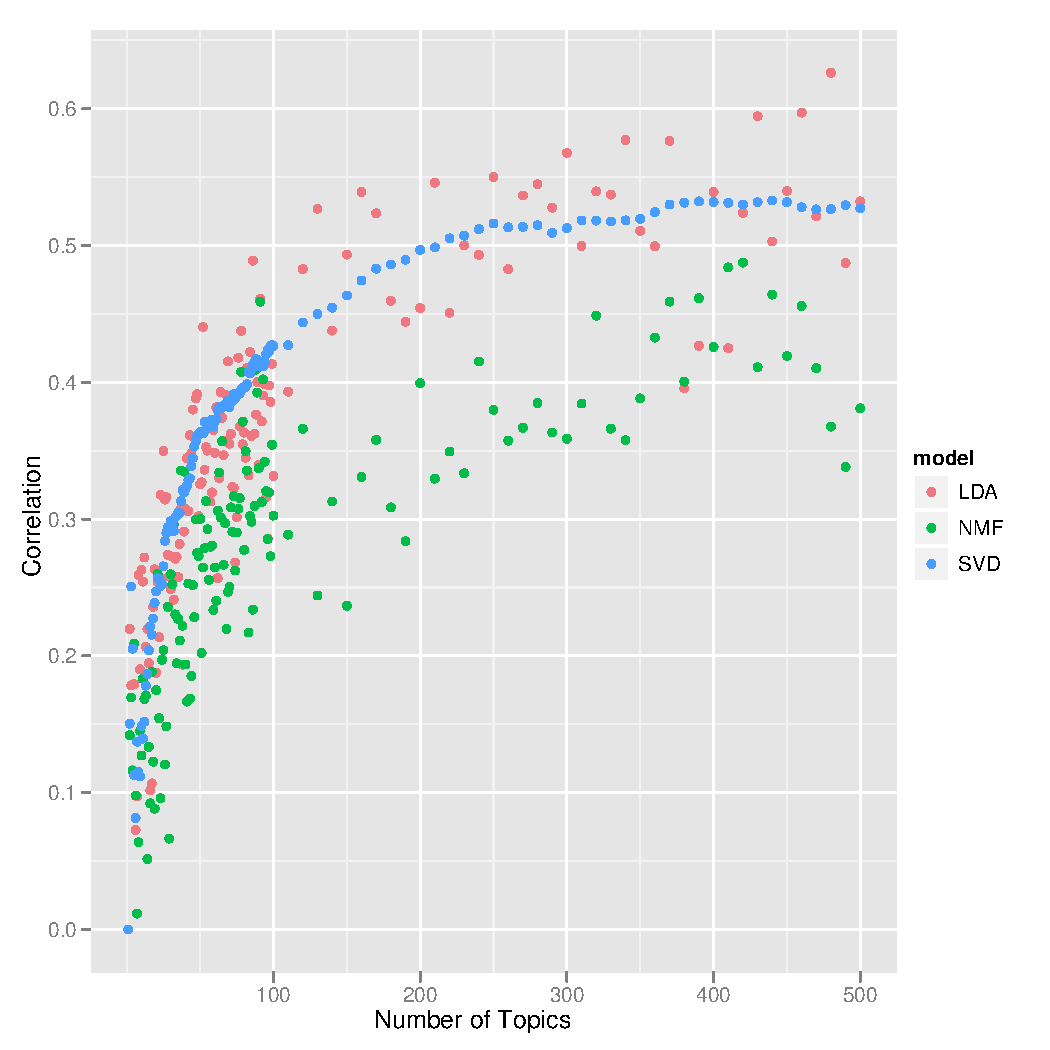
\includegraphics[width=\textwidth,height=.55\textwidth]{plots/rng_wordsim.pdf}
}
\only<3>{
\center
Correlation with WordSim-353 word pairs
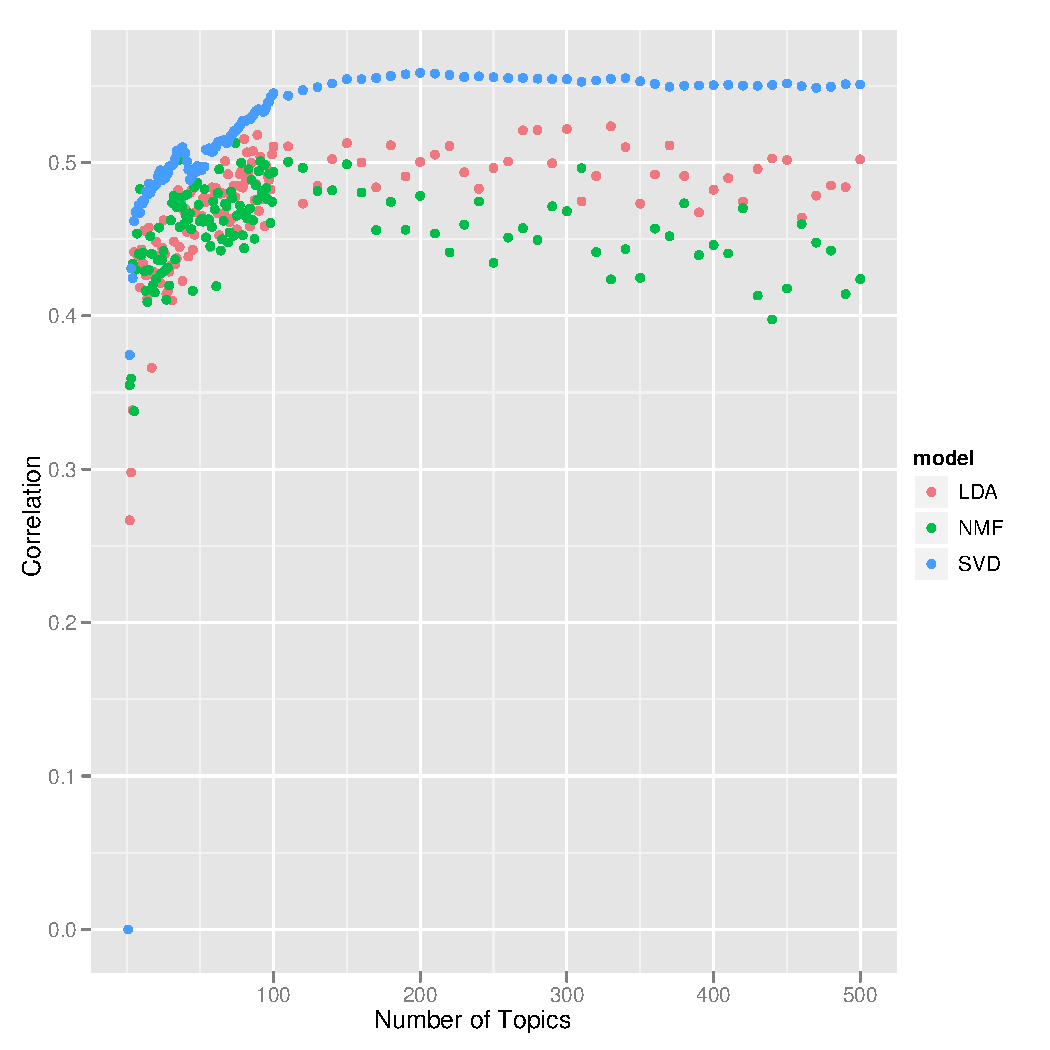
\includegraphics[width=\textwidth,height=.55\textwidth]{plots/353_wordsim.pdf}
}
\end{frame}

\subsection{Evaluating document categories}

\begin{frame}{Evaluating the latent document representations}

\only<1>{
\begin{block}{Categories on documents set a semantic scope}
Example: World News articles are related to each other, less so to Science
articles \\
Goal: Document representations should encode these differences
\end{block}

Setup:
\begin{itemize}
\item Train and Test a classifier using stratified 10-fold cross validation
\item Train with Bagged Ensembles of CART-decision trees
\item Compare proposed labels to known categories
\item Higher accuracy means better representation
\end{itemize}
}
\only<2>{
    \center
    Classification accuracy of latent document representations
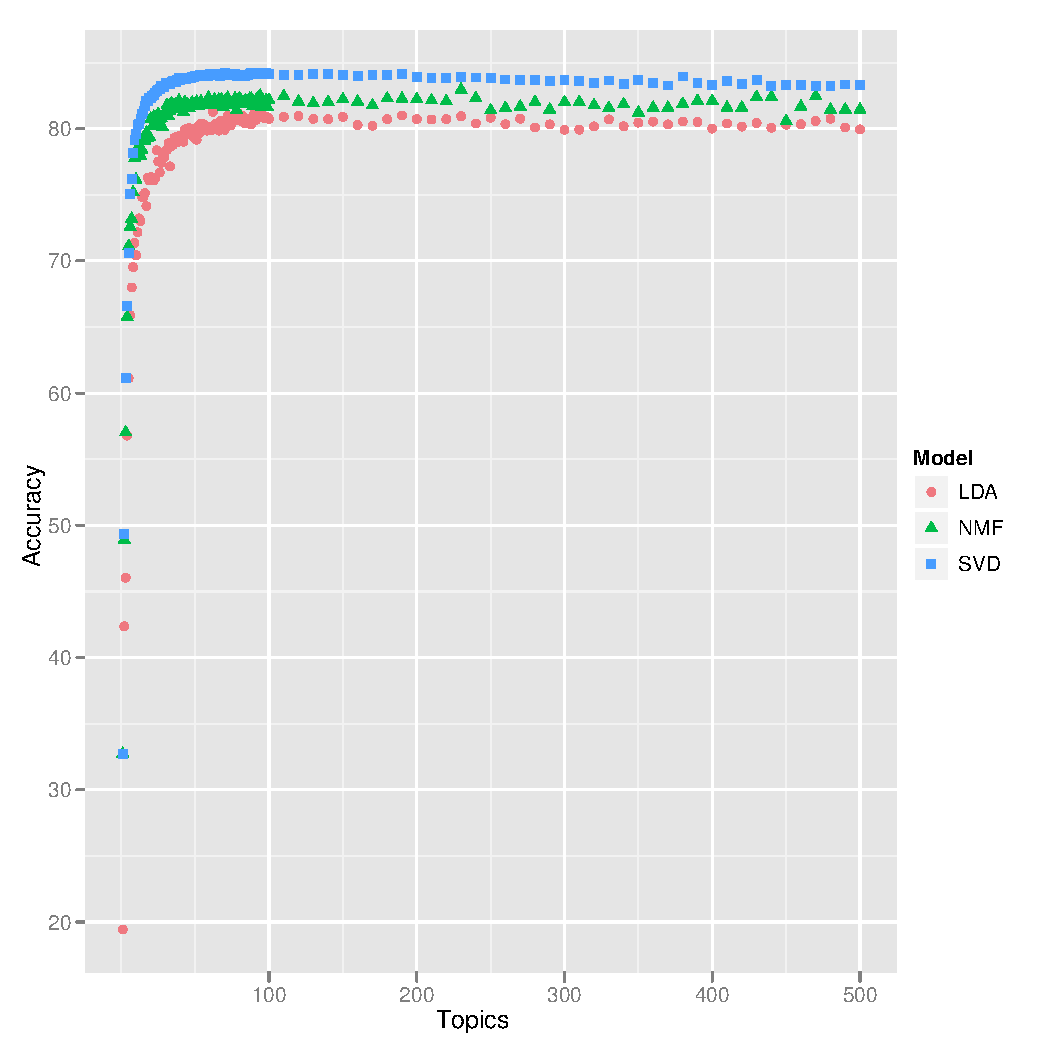
\includegraphics[width=\textwidth,height=.55\textwidth]{plots/avatar_classifier.pdf}
}
\only<3>{
    \center
    Correlation between feature ranking and UCI Topic Coherence
    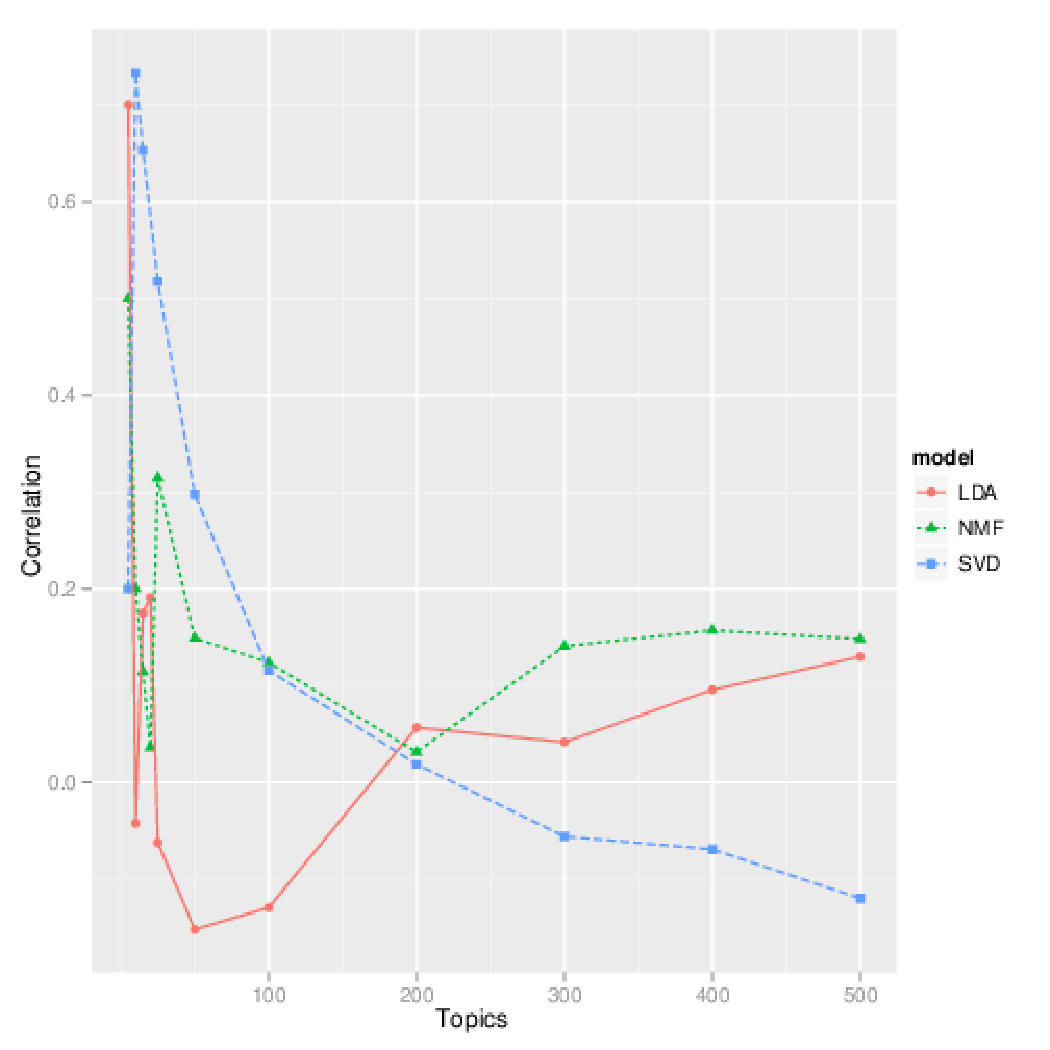
\includegraphics[width=\textwidth,height=.55\textwidth]{plots/uciNoSmoothing-ranks.pdf}
}
\only<4>{
    \center
    Classification Accuracy with more classifiers
    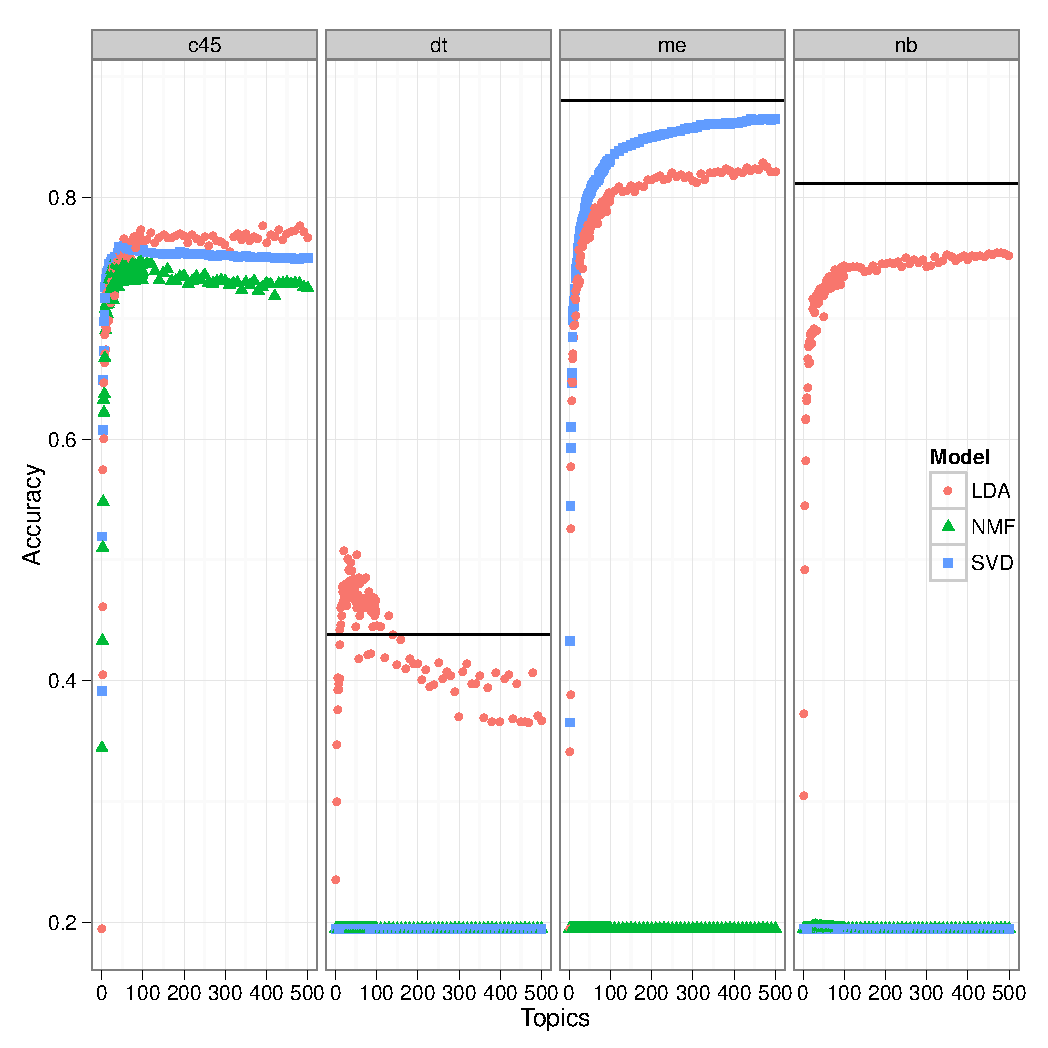
\includegraphics[width=\textwidth,height=.55\textwidth]{mallet-classifier-accuracy-topics.pdf}
}
\end{frame}

\section{Conclusions}

\begin{frame}{Topic Model Conclusions}
\begin{itemize}
\item Key Finding: Each model is tuned for a different task
\item SVD is better for finding compact, abstract representations
\item LDA is better for learning meaningful/understandable topics
\item NMF does moderately well on all tasks but never shines
\end{itemize}

\begin{block}{Take away point}
Pick your model based on your task and test for it carefully.  
\end{block}

\pause
 Lastly, Code to run experiments is provided on GitHub:
 https://github.com/fozziethebeat/TopicModelComparison \footnote{But the New
 York Times dataset isn't, see the LDC for that}
\end{frame}

\end{document}
